% Author: Izaak Neutelings (May 2021)
% Description:
%   Experimenting with finding the tangent to an ellipse
%   with the purpose of finding a nice way to draw a 3D cone.
\documentclass[border=3pt,tikz]{standalone}
\usepackage{amsmath}
\usepackage{mathtools} % for \eqcolon
\usepackage{physics}
\usepackage{siunitx}
\usepackage{xcolor}
\usepackage{etoolbox} %ifthen
\usepackage[outline]{contour} % glow around text
\usetikzlibrary{calc}
\usetikzlibrary{math} % for \tikzmath
\usetikzlibrary{angles,quotes} % for pic (angle labels)
\tikzset{>=latex} % for LaTeX arrow head
\contourlength{1.6pt}

\colorlet{myblue}{blue!70!black}
\colorlet{mygreen}{green!40!black}
\colorlet{myred}{red!65!black}
\tikzstyle{vector}=[->,very thick,myblue,line cap=round]
\tikzstyle{cone}=[thin,blue!50!black,fill=blue!50!black!30,fill opacity=0.8]

\newcommand\rightAngle[4]{
  \pgfmathanglebetweenpoints{\pgfpointanchor{#2}{center}}{\pgfpointanchor{#3}{center}}
  \coordinate (tmpRA) at ($(#2)+(\pgfmathresult+45:#4)$);
  %\draw[white,line width=0.6] ($(#2)!(tmpRA)!(#1)$) -- (tmpRA) -- ($(#2)!(tmpRA)!(#3)$);
  \draw[blue!40!black] ($(#2)!(tmpRA)!(#1)$) -- (tmpRA) -- ($(#2)!(tmpRA)!(#3)$);
}


\begin{document}


% TANGENT to CIRCLE - known: r, q
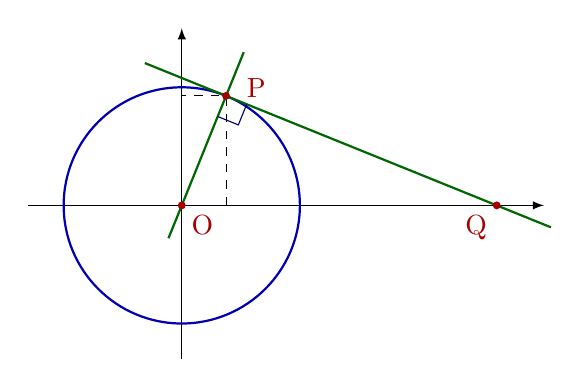
\begin{tikzpicture}
  \def\r{1.5} % radius
  \def\q{4} % distance center-external point q = |OQ|
  \def\x{{\r^2/\q}} % Q x coordinate
  \def\y{{\r*sqrt(1-(\r/\q)^2}} % Q y coordinate
  \coordinate (O) at (0,0); % circle center O
  \coordinate (Q) at (\q,0); % external point Q
  \coordinate (P) at (\x,\y); % point of tangency, P
  \draw[->] (0,-1.3*\r) -- (0,1.5*\r);
  \draw[->] (-1.3*\r,0) -- (\q+0.4*\r,0);
  \draw[dashed] (\x,0) |- (0,\y);
  \draw[myblue,thick] (O) circle(\r);
  \draw[mygreen,thick] ($(Q)!-0.2!(P)$) -- ($(Q)!1.3!(P)$);
  \draw[mygreen,thick] ($(O)!-0.3!(P)$) -- ($(O)!1.4!(P)$);
  \rightAngle{Q}{P}{O}{0.40}
  \fill[myred] (O) circle(0.05) node[below right] {O};
  \fill[myred] (Q) circle(0.05) node[below left] {Q};
  \fill[myred] (P) circle(0.05) node[above=3,right=4] {P};
\end{tikzpicture}


% TANGENT to ELLIPSE - known: a, b, q
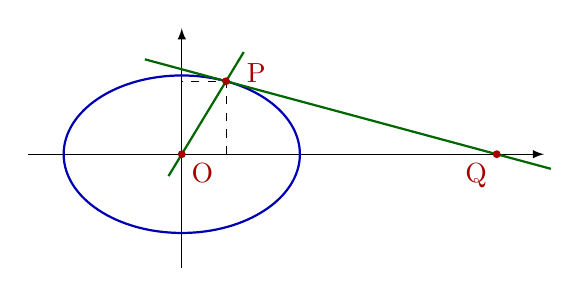
\begin{tikzpicture}
  \def\a{1.5} % horizontal radius
  \def\b{1.0} % vertical radius
  \def\q{4} % distance center-external point q = |OQ|
  \def\x{{\a^2/\q}} % x coordinate P
  \def\y{{\b*sqrt(1-(\a/\q)^2}} % y coordinate P
  \coordinate (O) at (0,0); % circle center O
  \coordinate (Q) at (\q,0); % external point Q
  \coordinate (P) at (\x,\y); % point of tangency, P
  \draw[->] (0,-\b-0.3*\a) -- (0,\b+0.4*\a);
  \draw[->] (-1.3*\a,0) -- (\q+0.4*\a,0);
  \draw[dashed] (\x,0) |- (0,\y);
  \draw[myblue,thick] (O) ellipse({\a} and {\b});
  \draw[mygreen,thick] ($(Q)!-0.2!(P)$) -- ($(Q)!1.3!(P)$);
  \draw[mygreen,thick] ($(O)!-0.3!(P)$) -- ($(O)!1.4!(P)$);
  \fill[myred] (O) circle(0.05) node[below right] {O};
  \fill[myred] (Q) circle(0.05) node[below left] {Q};
  \fill[myred] (P) circle(0.05) node[above=3,right=4] {P};
\end{tikzpicture}


% EQUATIONS, known: r (or a, b), q
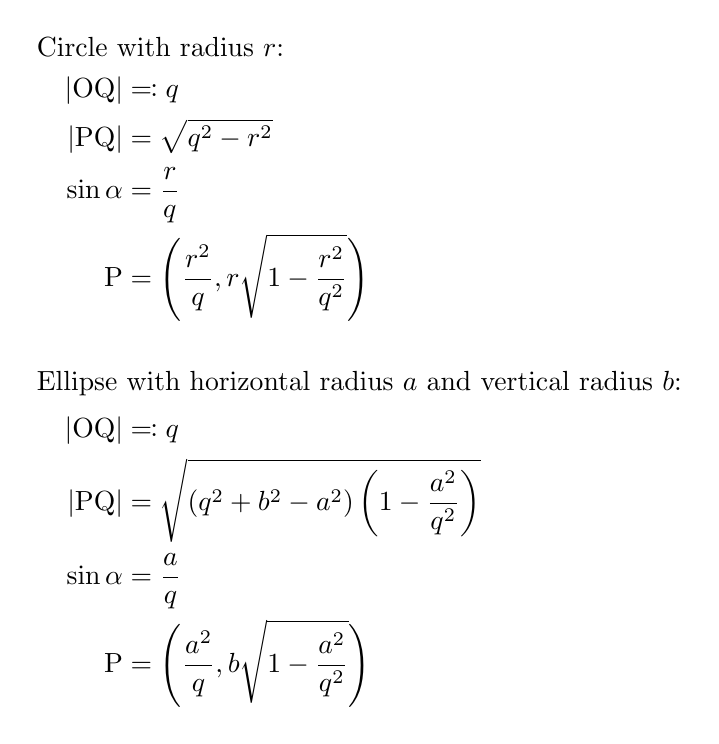
\begin{tikzpicture}[scale=1]
  \node[align=left] at (0,0) {
    Circle with radius $r$:\\[2mm]$\quad
    \begin{aligned}
      \abs{\mathrm{OQ}} &\eqqcolon q \\
      \abs{\mathrm{PQ}} &= \sqrt{q^2-r^2} \\
      \sin{\alpha} &= \frac{r}{q} \\
      \mathrm{P} &= \left( \frac{r^2}{q}, r\sqrt{1-\frac{r^2}{q^2}} \right) \\
    \end{aligned}$\\[6mm]
    Ellipse with horizontal radius $a$ and vertical radius $b$:\\[2mm]$\quad
    \begin{aligned}
      \abs{\mathrm{OQ}} &\eqqcolon q \\
      \abs{\mathrm{PQ}} &= \sqrt{\left(q^2+b^2-a^2\right)\left(1-\frac{a^2}{q^2}\right) } \\
      \sin{\alpha} &= \frac{a}{q} \\
      \mathrm{P} &= \left( \frac{a^2}{q}, b\sqrt{1-\frac{a^2}{q^2}} \right) \\
    \end{aligned}$};
\end{tikzpicture}


% TANGENT to CIRCLE - known: r, alpha
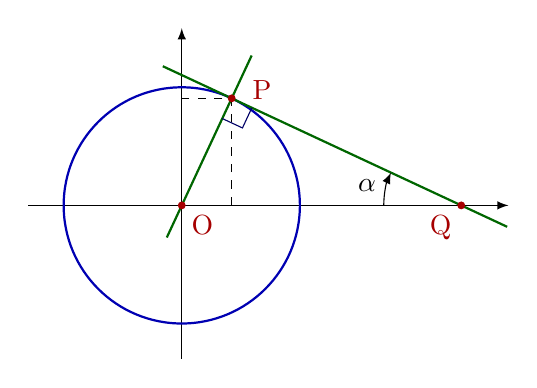
\begin{tikzpicture}
  \def\r{1.5} % radius
  \def\ang{25} % alpha angle
  \def\q{\r/sin(\ang)} % distance center-external point q = |OQ|
  \coordinate (O) at (0,0); % circle center O
  \coordinate (Q) at ({\q},0); % external point Q
  \coordinate (P) at (90-\ang:\r); % point of tangency, P
  \draw[->] (0,-1.3*\r) -- (0,1.5*\r);
  \draw[->] (-1.3*\r,0) -- ({\q+0.4*\r},0);
  \draw[dashed] ({\r*sin(\ang)},0) |- (0,{\r*cos(\ang)});
  \draw[myblue,thick] (O) circle(\r);
  \draw[mygreen,thick] ($(Q)!-0.2!(P)$) -- ($(Q)!1.3!(P)$);
  \draw[mygreen,thick] ($(O)!-0.3!(P)$) -- ($(O)!1.4!(P)$);
  \rightAngle{Q}{P}{O}{0.40}
  \fill[myred] (O) circle(0.05) node[below right] {O};
  \fill[myred] (Q) circle(0.05) node[below left] {Q};
  \fill[myred] (P) circle(0.05) node[above=3,right=4] {P};
  \draw pic[<-,"$\alpha$"{above=1,left=0},draw=black,angle radius=28,angle eccentricity=1.0]
    {angle = P--Q--O};
\end{tikzpicture}


% TANGENT to ELLIPSE - known: a, b, alpha
\foreach \b in {1.0,2.0}{ % vertical radius
\foreach \ang in {25}{ % alpha angle
\begin{tikzpicture}
  \def\a{1.5} % horizontal radius
  %\def\b{1.0} % vertical radius
  %\def\ang{25} % alpha angle
  \def\q{\a/sin(\ang)} % distance center-external point q = |OQ|
  \coordinate (O) at (0,0); % circle center O
  \coordinate (Q) at ({\q},0); % external point Q
  \coordinate (P) at (90-\ang:{\a} and {\b}); % point of tangency, P
  \draw[->] (0,-\b-0.3*\a) -- (0,\b+0.5*\a);
  \draw[->] (-1.3*\a,0) -- ({\q+0.4*\a},0);
  \draw[dashed] ({\a*sin(\ang)},0) |- (0,{\b*cos(\ang)});
  \draw[myblue,thick] (O) ellipse({\a} and {\b});
  \draw[mygreen,thick] ($(Q)!-0.2!(P)$) -- ($(Q)!1.3!(P)$);
  \draw[mygreen,thick] ($(O)!-0.3!(P)$) -- ($(O)!1.4!(P)$);
  \fill[myred] (O) circle(0.05) node[below right] {O};
  \fill[myred] (Q) circle(0.05) node[below left] {Q};
  \fill[myred] (P) circle(0.05) node[above=3,right=4] {P};
  \draw pic[<-,"$\alpha$"{above=1,left=0},draw=black,angle radius=28,angle eccentricity=1.0]
    {angle = P--Q--O};
  \node[right,align=left] at ({0.85*\q},\b+0.6)
    {$\begin{aligned}
       a &= \a\\
       b &= \b\\
       \alpha &= \SI{\ang}{\degree}
     \end{aligned}$};
\end{tikzpicture}
}}


% EQUATIONS, known: r (or a, b), alpha
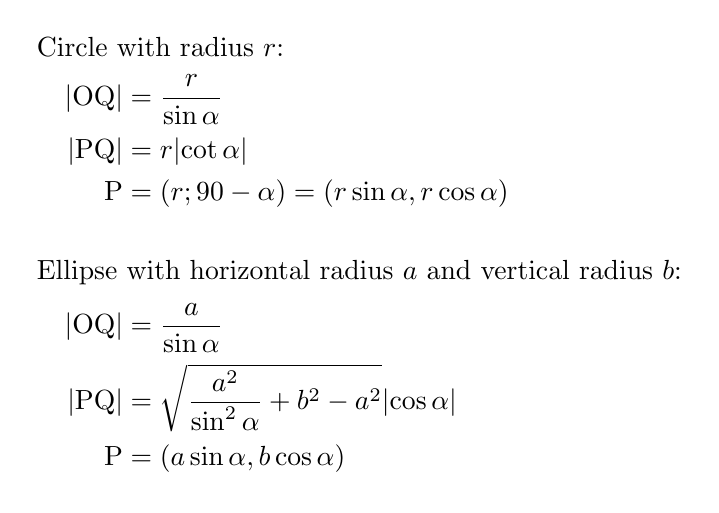
\begin{tikzpicture}[scale=1]
  \node[align=left] at (0,0) {
    Circle with radius $r$:\\[2mm]$\quad
    \begin{aligned}
      \abs{\mathrm{OQ}} &= \frac{r}{\sin\alpha} \\
      \abs{\mathrm{PQ}} &= r\abs{\cot\alpha} \\
      \mathrm{P} &= (r;90-\alpha) = (r\sin\alpha,r\cos\alpha) \\
    \end{aligned}$\\[6mm]
    Ellipse with horizontal radius $a$ and vertical radius $b$:\\[2mm]$\quad
    \begin{aligned}
      \abs{\mathrm{OQ}} &= \frac{a}{\sin\alpha} \\
      \abs{\mathrm{PQ}} &= \sqrt{\frac{a^2}{\sin^2\alpha}+b^2-a^2}\abs{\cos\alpha} \\
      \mathrm{P} &= (a\sin\alpha,b\cos\alpha) \\
    \end{aligned}$};
\end{tikzpicture}


% TANGENT to CIRCLE - known: vector, alpha
\begin{tikzpicture}
  \def\ang{20} % alpha angle
  \coordinate (O) at (0,0); % circle center O
  \coordinate (Q) at (4,1); % external point Q
  \tikzmath{
    coordinate \C;
    \C = (O)-(Q);
    \r = veclen(\Cx,\Cy)*sin(\ang);
  }
  \pgfmathanglebetweenpoints{\pgfpointanchor{Q}{center}}{\pgfpointanchor{O}{center}}
  \edef\vecang{\pgfmathresult}
  \coordinate (P) at ($(O)+({\vecang-(90+\ang)}:\r pt)$); % point of tangency, P
  \draw[myblue,thick] (O) circle(\r pt);
  \draw[mygreen,thick] ($(Q)!-0.2!(P)$) -- ($(Q)!1.3!(P)$);
  \draw[mygreen,thick] ($(O)!-0.3!(P)$) -- ($(O)!1.4!(P)$);
  \draw ($(O)!-0.5!(Q)$) -- ($(O)!1.3!(Q)$);
  \draw[vector] (Q) -- (O);
  \rightAngle{Q}{P}{O}{0.40}
  \fill[myred] (O) circle(0.05) node[below right] {O};
  \fill[myred] (Q) circle(0.05) node[below left] {Q};
  \fill[myred] (P) circle(0.05) node[above right=1] {P};
  \draw pic[<-,"$\alpha$"{above=1,left=0},draw=black,angle radius=28,angle eccentricity=1.0]
    {angle = P--Q--O};
\end{tikzpicture}


% TANGENT to ELLIPSE - known: vector, angle, a/b
\begin{tikzpicture}
  \def\ang{20} % alpha angle
  \def\e{0.4} % x scale
  \coordinate (O) at (0,0); % circle center O
  \coordinate (Q) at (4,1); % external point Q
  \pgfmathanglebetweenpoints{\pgfpointanchor{Q}{center}}{\pgfpointanchor{O}{center}}
  \edef\vecang{\pgfmathresult} % angle of vector QO
  \tikzmath{
    coordinate \C;
    \C = (O)-(Q);
    \x = veclen(\Cx,\Cy)*\e*sin(\ang)^2; % x coordinate P
    \y = tan(\ang)*(veclen(\Cx,\Cy)-\x); % y coordinate P
    \a = veclen(\Cx,\Cy)*sqrt(\e)*sin(\ang); % vertical radius
    \b = veclen(\Cx,\Cy)*tan(\ang)*sqrt(1-\e*sin(\ang)^2); % horizontal radius
  }
  \coordinate (P) at ($(O)+(\vecang-180:\x pt)+(\vecang-90:\y pt)$); % point of tangency, P
  \draw[myblue,thick,rotate=\vecang] (O) ellipse({\a pt} and {\b pt});
  \draw[mygreen,thick] ($(Q)!-0.2!(P)$) -- ($(Q)!1.3!(P)$);
  \draw[mygreen,thick] ($(O)!-0.3!(P)$) -- ($(O)!1.4!(P)$);
  \draw ($(O)!-0.5!(Q)$) -- ($(O)!1.3!(Q)$);
  \draw[vector] (Q) -- (O);
  \fill[myred] (O) circle(0.05) node[below right] {O};
  \fill[myred] (Q) circle(0.05) node[below left] {Q};
  \fill[myred] (P) circle(0.05) node[above right=1] {P};
  \draw pic[<-,"$\alpha$"{above=1,left=0},draw=black,angle radius=28,angle eccentricity=1.0]
    {angle = P--Q--O};
\end{tikzpicture}


% CONE
\foreach \ang in {10,20}{ % alpha angle
\foreach \e in {0.05,0.5}{ % x scale
\begin{tikzpicture}
  %\def\ang{10} % alpha angle
  %\def\e{0.3} % x scale
  \coordinate (O) at (0,0);
  \coordinate (V) at (5,2);
  \pgfmathanglebetweenpoints{\pgfpointanchor{O}{center}}{\pgfpointanchor{V}{center}}
  \edef\vecang{\pgfmathresult} % angle of vector OV
  \tikzmath{
    coordinate \C;
    \C = (O)-(V);
    \x = veclen(\Cx,\Cy)*\e*sin(\ang)^2; % x coordinate P
    \y = tan(\ang)*(veclen(\Cx,\Cy)-\x); % y coordinate P
    \a = veclen(\Cx,\Cy)*sqrt(\e)*sin(\ang); % vertical radius
    \b = veclen(\Cx,\Cy)*tan(\ang)*sqrt(1-\e*sin(\ang)^2); % horizontal radius
    \angb = acos(sqrt(\e)*sin(\ang)); % angle of P in ellipse
  }
  \coordinate (V') at ($(V)+(\vecang:1.15*\a pt + 10 pt)$); %($(O)!{1/cos(\ang)^2}!(V)$);
  \coordinate (R) at ($(V)+(\vecang-180:\x pt)+(\vecang-90:\y pt)$); % tangency
  \coordinate (L) at ($(V)+(\vecang-180:\x pt)+(\vecang+90:\y pt)$); % tangency
  %\coordinate (R') at ($(V)+(\vecang-90:\b pt)$); % tangency
  %\coordinate (L') at ($(V)+(\vecang+90:\b pt)$); % tangency
  \draw[cone,rotate=\vecang]
    (V) ellipse({\a pt} and {\b pt});
  \draw[vector] (O) -- (V');
  \draw[cone,rotate=\vecang]
    (L) arc(180-\angb:180+\angb:{\a pt} and {\b pt}) -- (O) -- cycle;
  \draw[mygreen,thick] (O) -- (L);
  \draw[mygreen,thick] (O) -- (R);
  \fill[myred] (O) circle(0.05) node[below left] {O};
  \fill[myred] (V) circle(0.05) node[below right] {V};
  \fill[myred] (V') circle(0.05) node[below right] {V$'$};
  \fill[myred] (L) circle(0.05) node[above left=-1] {L};
  \fill[myred] (R) circle(0.05) node[below=0] {R};
  %\fill[myred] (L') circle(0.05) node[above right=-1] {L$'$};
  %\fill[myred] (R') circle(0.05) node[below right] {R$'$};
  \node[right,align=left] at (-0.2,2.5) {$\begin{aligned}
       \alpha &= \SI{\ang}{\degree} \\
       \theta &= \angb \\
       e &= \e
     \end{aligned}$};
\end{tikzpicture}
}}


\end{document}